\section{A First Approach by Merging}
\label{tree:xy:merge}

In our first approach, we sort \XY using half
the comparisons required by the \ITLB for Sorting. We do so by exploiting the
\emph{poset structure of \XY}.
We thus solve this problem in a strictly faster way than sorting a set of size
\(n^2\)
with a classical sorting algorithm, by taking advantage of some of the information we already have.

The \ITLB for sorting a set of size \(N\) is
\begin{displaymath}
\log N! \simeq N \log N - 1.44 N + \BigO{\log N}.
\end{displaymath}
Sorting \XY without information requires thus at least
\begin{displaymath}
\log n^2! \simeq 2 n^2 \log n - 1.44 n^2 + \BigO{\log n}
\end{displaymath}
queries.
In the next paragraphs we show that it is possible to sort \XY
with at most \(n^2 \log n + \BigO{n^2}\).

\begin{figure}
\centering
\begin{subfigure}[t]{0.47\textwidth}
\centering
	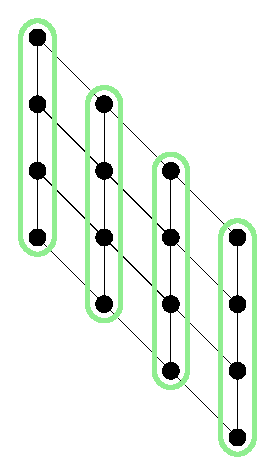
\includegraphics[width=0.4\textwidth]{fig/x+y/poset/chains}
	\subcaption{Balanced selection of disjoint chains in the \XY poset.}
	\label{fig:xy:poset:chains}
\end{subfigure}
~
\begin{subfigure}[t]{0.47\textwidth}
\centering
	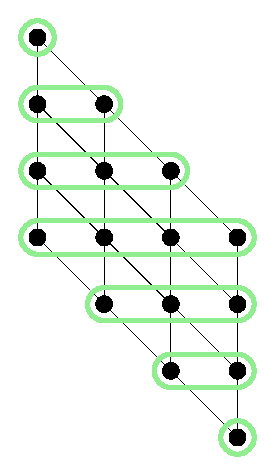
\includegraphics[width=0.4\textwidth]{fig/x+y/poset/antichains}
	\subcaption{Maximal antichains in the \XY poset.}
	\label{fig:xy:poset:antichains}
\end{subfigure}
\caption{Structure of the \XY poset.}
\label{fig:xy:poset:diagrams}
\end{figure}

\begin{figure}
\centering
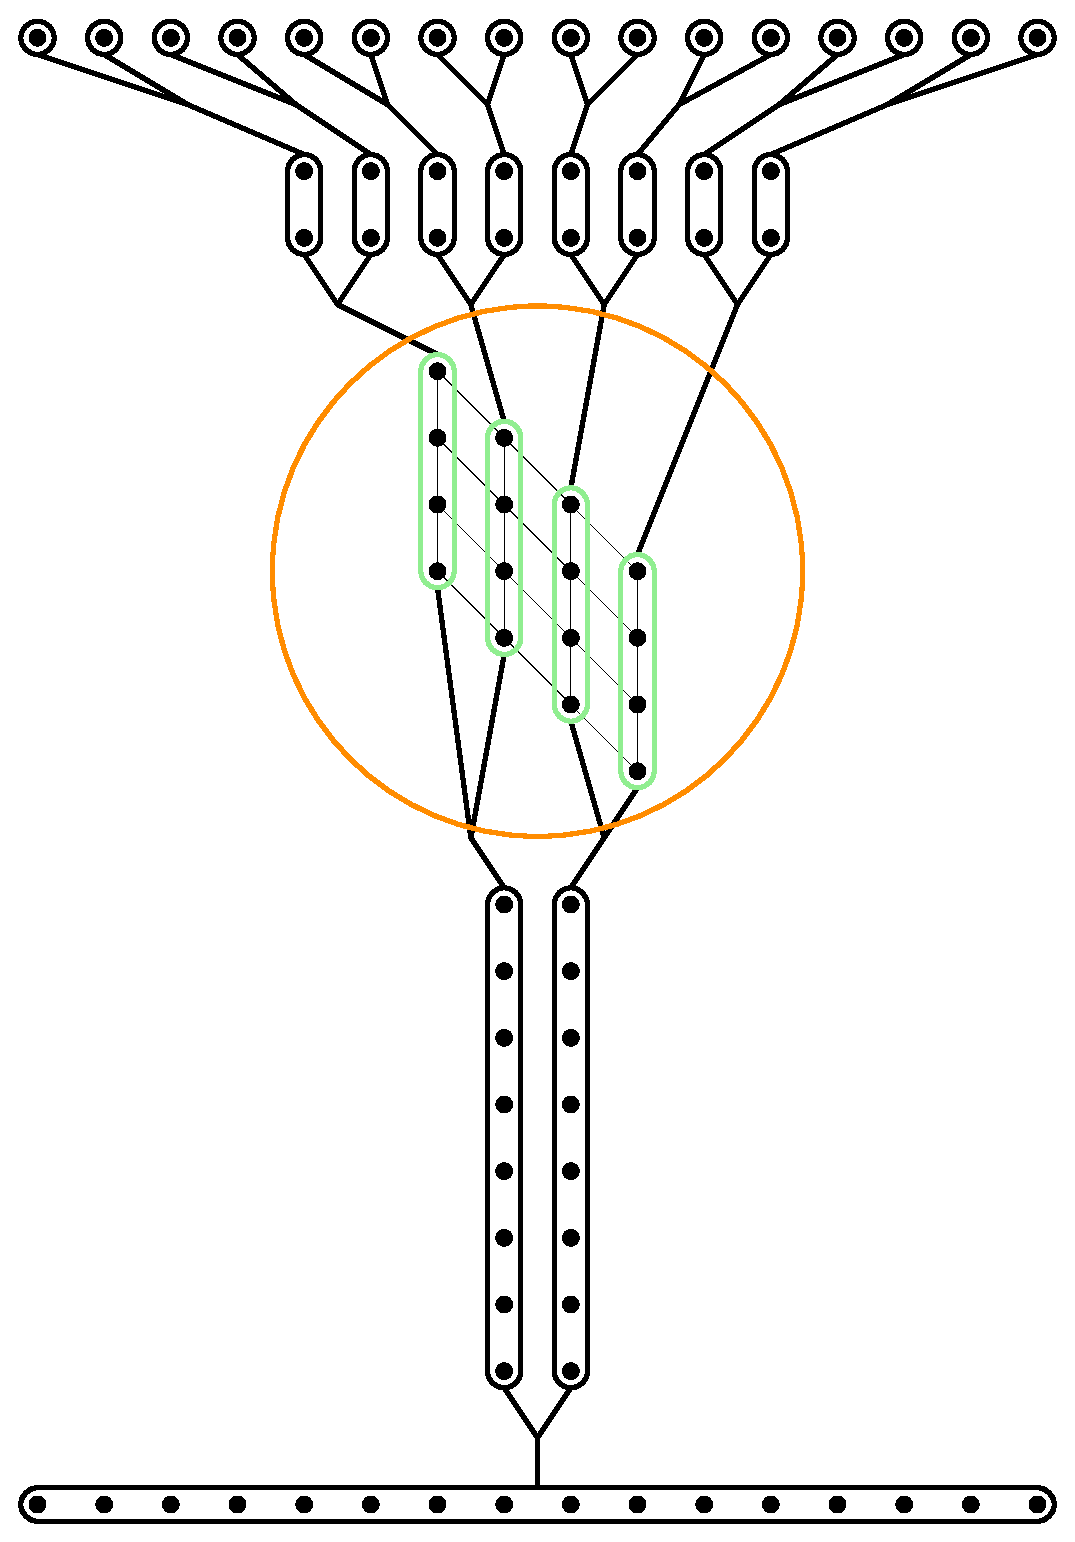
\includegraphics[width=0.5\textwidth,angle=90]{fig/x+y/poset/mergexy}
\caption{Resolution of the \mergesort algorithm. The circled part
corresponds to the starting point of our first Sorting \XY algorithm on an
input of size \(4 \times 4\).}
\label{fig:xy:poset:mergexy}
\end{figure}

We define the poset structure of \XY (or simply the \XY poset) to be the poset
containing the information that we can extract from the transitivity of the
total order on \(X \cup Y\). If we only exploit the fact that
\begin{displaymath}
X_i \le X_{i'} \land Y_j \le \Y_{j'} \implies X_i + Y_j \le X_{i'} + Y_{j'}
\end{displaymath}
we obtain the poset represented by the Hasse diagram (\Cref{tree:poset:hasse})
in \ref{fig:related:xy} (\Cref{tree:related:xy}).
Chains and antichains
in the \XY poset obey a regular pattern. To illustrate this, we take the $4 \times 4$
\XY poset. We highlight a possible selection of disjoint chains in
\ref{fig:xy:poset:chains} and the set of maximal antichains found by a greedy
algorithm in \ref{fig:xy:poset:antichains}.

To illustrate our approach, we show in \ref{fig:xy:poset:mergexy} the steps of
the \mergesort algorithm on an input of size \(16\).
What is highlighted in \ref{fig:xy:poset:mergexy} is a subset of the
information we have when knowing the structure of \XY, \ie the chains of
\ref{fig:xy:poset:chains}. It means that the step we
highlighted can be attained without any comparison if the set to sort is \XY
and if we know its structure. Note that if not known a priori, this structure
can be revealed for the cost of \(2n \log n + \BigO{n}\) comparisons, using a standard \(n
\log n + \BigO{n}\) comparison sorting algorithm to sort sets \(X\) and \(Y\).

In \mergesort there are $\log N$ steps. At step $i$ we have
built $2^{i}$ total orders on disjoint subsets of size $2^{\log N - i}$. Since
the step represented in \ref{fig:xy:poset:mergexy} shows $n$ total orders on
disjoint subsets of size $n$, and that the total number of elements in \XY is
$N = n^2$ we can conclude that \ref{fig:xy:poset:mergexy} shows us step
$\sfrac{1}{2} \log N$. Indeed, we give here an example where \(n\) is a power
of \(2\)
but it is not difficult to convince oneself that starting
the algorithm at the median step
saves us half the comparisons, for \(n\) large enough. However we rely on the
results we gave in \Cref{tree:merging:kgeq3} to prove that it is possible to
reuse this subset of the partial information optimally.
\begin{theorem}[A first upper bound for Sorting \XY]
Sorting \XY requires at most \(n^2 \log n + \BigO{n}\) queries to be made.
\end{theorem}
\begin{proof}
Note that if \(\log n^2!\) is the total amount of information to retrieve,
then recycling the information contained in the \(n\) chains of length \(n\)
gives us \(n \cdot \log n! \simeq n^2 \log n - \BigO{n^2}\) bits of information already in our
possession. We saw in \Cref{tree:merging:kgeq3} that we can reuse this information optimally using
the Huffman code based merging algorithm.
\end{proof}

Since this algorithm reuses only a fraction of the available information, the
question of the optimality of this approach remains. We give an answer to this
question in the next sections.
